\renewcommand{\theequation}{\theenumi}
\begin{enumerate}[label=\thesection.\arabic*.,ref=\thesection.\theenumi]
\numberwithin{equation}{enumi}
\item The figure for the parallelogram obtained in the question looks like Fig. \ref{fig:parallelogram1}.
%with angles $\phase{ A},\phase{ C}$ and $\phase{ B}$ and sides $a, b$ and $c$.  The unique feature of this triangle is $\phase{ C}$ which is defined to be $90\degree$.
with with vectors \textbf{a} and \textbf{b}.


%\renewcommand{\thefigure}{\theenumi.\arabic{figure}}
\begin{figure}[!ht]
\centering
\resizebox{\columnwidth}{!}{%
%
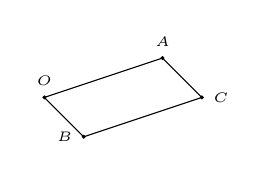
\begin{tikzpicture}
%[scale=0.5,>=stealth,point/.style={draw,circle,fill = green,inner sep=0.1pt},]
[scale=0.5,>=stealth, point/.style={draw,circle,fill = black,inner sep=0.1pt}]


%%
%%%Triangle sides
\def\a{4.12}
\def\b{4.47}
%\def\c{sqrt(\a^2+\c^2)}
\def\c{8.06}
%%
%%
%%
%%%Labeling points
%\node (A) at (0,\b)[point,label=above right:$A$] {};
%\node (B) at (\a, 0)[point,label=below left:$B$] {};
%\node (C) at (0, 0)[point,label=below right:$C$] {};
%\node (M) at (\a*0.5,\b*0.5)[point,label=above:$M$] {};
%\node (D) at (\a,\b)[point,label=above right:$D$] {};
%%
%%
%%%Drawing triangle ABC
%\draw (A) -- node[below] {$\textrm{}$} (B) -- node[left] {$\textrm{a}$} (C) -- node[above,xshift=5mm] {$\textrm{b}$} (A);
%%
%%%Joining CD
%\draw (C)--(D);
%%%Joining BD
%\draw (B)--(D);
%%
%%%Drawing and marking angles
%%\tkzMarkAngle[fill=orange!40,size=0.5cm,mark=](A,M,C)
%%\tkzMarkAngle[fill=orange!40,size=0.5cm,mark=](B,M,D)
%%\tkzMarkAngle[fill=green!40,size=0.5cm,mark=](A,B,C)
%%\tkzMarkRightAngle[fill=blue!20,size=.2](A,C,B)
%%\tkzMarkRightAngle[fill=blue!20,size=.2](D,B,C)
%%\tkzLabelAngle[pos=0.65](A,M,C){$\theta$}
%%\tkzLabelAngle[pos=0.65](B,M,D){$\theta$}
%%\tkzLabelAngle[pos=0.65](A,B,C){$\alpha$}
%%


% the coordinates of the vertices
\coordinate (A) at (3,1);
\coordinate (B) at (1,-1);
\coordinate (C) at (4,0);
\coordinate (O) at (0,0);



%\coordinate (M) at (3.5,-4);
%\coordinate (N) at (4,0);
%\coordinate (P) at (4.5,-2);

% the axis
\draw[thin,scale=0,-] (-1,0) -- (5.5,0);
\draw[thin,scale=0,-] (0,-2.5) -- (0,2.5);

% the edges of the triangle
\draw (O) -- (A) -- (C) -- (B)-- cycle;
%\draw[-] (B) -- (P) ;
%\draw[-] (A) -- (N) ;
%\draw[-] (C) -- (M) ;

% labelling the vertices
%\node (A) at (4,-6)[point,label=above right:$A$] {};
\node[point,label={above:\tiny $A$}] at (A) {};
\node[point,label={left:\tiny $B$}] at (B) {};
\node[point,label={right:\tiny $C$}] at (C) {};
\node[point,label={above:\tiny $O$}] at (O) {};
%\node (M) at (3.5,-4)[point,label=left:\tiny $M$]{};
%\node (N) at (4,0)[point,label=above:\tiny $N$] {};
%\node (P) at (4.5,-2)[point,label=right:\tiny $P$] {};

% the arcs for the angles
%\begin{scope}[black]
%\draw[->]
%  (1,0) +(0:0.5cm) arc [radius=1cm,start angle=0,end angle=41] node[midway,right] {$\alpha$};
%\draw[->]
%  (0.5,0) +(0:0.25cm) arc [radius=0.75cm,start angle=0,end angle=122] node[midway,above] {$\beta$};
%\end{scope}
%
\end{tikzpicture}
%



%\begin{tikzpicture}[scale=.5]
%  \tkzDefPoint(4,-6){A} \tkzDefPoint(3,-2){B}
%  %\tkzDrawCircle[R,dashed](A,7 cm) \tkzDrawCircle[R,dashed](B,13 cm)
%  \tkzInterCC[R](A,4.12 cm)(B,4.47 cm) \tkzGetPoints{C}{D}
%  \tkzDrawPolygon(A,B,C)
%  \tkzCompasss(A,C B,C)
%  \tkzLabelSegment[below](A,B){$4.12$ cm}
%  \tkzLabelSegment[above left](A,C){$4.47$ cm}
%  \tkzLabelSegment[above right](B,C){$8.06$ cm}
%  \tkzDrawPoints[color=red](C)
%  \tkzDrawPoints[color=blue](A,B)
%\end{tikzpicture}
}
\caption{Parallelogram by Latex-Tikz}
\label{fig:parallelogram1}	
\end{figure}
%
%
%\renewcommand{\thefigure}{\theenumi}
%
\item List the design parameters for construction
\label{const:table1}
\\
\solution See Table. \ref{table:table1}. 
%
\begin{table}[ht!]
\centering
\begin{tabular}{ |p{3cm}|p{3cm}|  }
%\hline
% \multicolumn{2}{|c|}{Initial Input Values.} \\
\hline
Parameters & Values \\
\hline
%OA (a) & 4\\
OA $(\vec{a}) $ & $$\begin{pmatrix}3\\1\\4\end{pmatrix} $$\\
\hline
OB $(\vec{b}) $ & $$\begin{pmatrix}1\\-1\\1\end{pmatrix} $$\\
\hline
%$\phase{(ACB)$ & $90^{\circ}$ \\
%\hline
\end{tabular}
%%%%%%%%%%%%%%%%%%%%%%%%%%%%%%%%%%%%%%%%%%%%%%%%%%%%%%%%%%%%%%%%%%%%%%%
%%                                                                  %%
%%  This is the header of a LaTeX2e file exported from Gnumeric.    %%
%%                                                                  %%
%%  This file can be compiled as it stands or included in another   %%
%%  LaTeX document. The table is based on the longtable package so  %%
%%  the longtable options (headers, footers...) can be set in the   %%
%%  preamble section below (see PRAMBLE).                           %%
%%                                                                  %%
%%  To include the file in another, the following two lines must be %%
%%  in the including file:                                          %%
%%        \def\inputGnumericTable{}                                 %%
%%  at the beginning of the file and:                               %%
%%        \input{name-of-this-file.tex}                             %%
%%  where the table is to be placed. Note also that the including   %%
%%  file must use the following packages for the table to be        %%
%%  rendered correctly:                                             %%
%%    \usepackage[latin1]{inputenc}                                 %%
%%    \usepackage{color}                                            %%
%%    \usepackage{array}                                            %%
%%    \usepackage{longtable}                                        %%
%%    \usepackage{calc}                                             %%
%%    \usepackage{multirow}                                         %%
%%    \usepackage{hhline}                                           %%
%%    \usepackage{ifthen}                                           %%
%%  optionally (for landscape tables embedded in another document): %%
%%    \usepackage{lscape}                                           %%
%%                                                                  %%
%%%%%%%%%%%%%%%%%%%%%%%%%%%%%%%%%%%%%%%%%%%%%%%%%%%%%%%%%%%%%%%%%%%%%%



%%  This section checks if we are begin input into another file or  %%
%%  the file will be compiled alone. First use a macro taken from   %%
%%  the TeXbook ex 7.7 (suggestion of Han-Wen Nienhuys).            %%
\def\ifundefined#1{\expandafter\ifx\csname#1\endcsname\relax}


%%  Check for the \def token for inputed files. If it is not        %%
%%  defined, the file will be processed as a standalone and the     %%
%%  preamble will be used.                                          %%
\ifundefined{inputGnumericTable}

%%  We must be able to close or not the document at the end.        %%
	\def\gnumericTableEnd{\end{document}}


%%%%%%%%%%%%%%%%%%%%%%%%%%%%%%%%%%%%%%%%%%%%%%%%%%%%%%%%%%%%%%%%%%%%%%
%%                                                                  %%
%%  This is the PREAMBLE. Change these values to get the right      %%
%%  paper size and other niceties.                                  %%
%%                                                                  %%
%%%%%%%%%%%%%%%%%%%%%%%%%%%%%%%%%%%%%%%%%%%%%%%%%%%%%%%%%%%%%%%%%%%%%%

	\documentclass[12pt%
			  %,landscape%
                    ]{report}
       \usepackage[latin1]{inputenc}
       \usepackage{fullpage}
       \usepackage{color}
       \usepackage{array}
       \usepackage{longtable}
       \usepackage{calc}
       \usepackage{multirow}
       \usepackage{hhline}
       \usepackage{ifthen}

	\begin{document}


%%  End of the preamble for the standalone. The next section is for %%
%%  documents which are included into other LaTeX2e files.          %%
\else

%%  We are not a stand alone document. For a regular table, we will %%
%%  have no preamble and only define the closing to mean nothing.   %%
    \def\gnumericTableEnd{}

%%  If we want landscape mode in an embedded document, comment out  %%
%%  the line above and uncomment the two below. The table will      %%
%%  begin on a new page and run in landscape mode.                  %%
%       \def\gnumericTableEnd{\end{landscape}}
%       \begin{landscape}


%%  End of the else clause for this file being \input.              %%
\fi

%%%%%%%%%%%%%%%%%%%%%%%%%%%%%%%%%%%%%%%%%%%%%%%%%%%%%%%%%%%%%%%%%%%%%%
%%                                                                  %%
%%  The rest is the gnumeric table, except for the closing          %%
%%  statement. Changes below will alter the table's appearance.     %%
%%                                                                  %%
%%%%%%%%%%%%%%%%%%%%%%%%%%%%%%%%%%%%%%%%%%%%%%%%%%%%%%%%%%%%%%%%%%%%%%

\providecommand{\gnumericmathit}[1]{#1} 
%%  Uncomment the next line if you would like your numbers to be in %%
%%  italics if they are italizised in the gnumeric table.           %%
%\renewcommand{\gnumericmathit}[1]{\mathit{#1}}
\providecommand{\gnumericPB}[1]%
{\let\gnumericTemp=\\#1\let\\=\gnumericTemp\hspace{0pt}}
 \ifundefined{gnumericTableWidthDefined}
        \newlength{\gnumericTableWidth}
        \newlength{\gnumericTableWidthComplete}
        \newlength{\gnumericMultiRowLength}
        \global\def\gnumericTableWidthDefined{}
 \fi
%% The following setting protects this code from babel shorthands.  %%
 \ifthenelse{\isundefined{\languageshorthands}}{}{\languageshorthands{english}}
%%  The default table format retains the relative column widths of  %%
%%  gnumeric. They can easily be changed to c, r or l. In that case %%
%%  you may want to comment out the next line and uncomment the one %%
%%  thereafter                                                      %%
\providecommand\gnumbox{\makebox[0pt]}
%%\providecommand\gnumbox[1][]{\makebox}

%% to adjust positions in multirow situations                       %%
\setlength{\bigstrutjot}{\jot}
\setlength{\extrarowheight}{\doublerulesep}

%%  The \setlongtables command keeps column widths the same across  %%
%%  pages. Simply comment out next line for varying column widths.  %%
\setlongtables

\setlength\gnumericTableWidth{%
	56pt+%
	33pt+%
0pt}
\def\gumericNumCols{2}
\setlength\gnumericTableWidthComplete{\gnumericTableWidth+%
         \tabcolsep*\gumericNumCols*2+\arrayrulewidth*\gumericNumCols}
\ifthenelse{\lengthtest{\gnumericTableWidthComplete > \linewidth}}%
         {\def\gnumericScale{\ratio{\linewidth-%
                        \tabcolsep*\gumericNumCols*2-%
                        \arrayrulewidth*\gumericNumCols}%
{\gnumericTableWidth}}}%
{\def\gnumericScale{1}}

%%%%%%%%%%%%%%%%%%%%%%%%%%%%%%%%%%%%%%%%%%%%%%%%%%%%%%%%%%%%%%%%%%%%%%
%%                                                                  %%
%% The following are the widths of the various columns. We are      %%
%% defining them here because then they are easier to change.       %%
%% Depending on the cell formats we may use them more than once.    %%
%%                                                                  %%
%%%%%%%%%%%%%%%%%%%%%%%%%%%%%%%%%%%%%%%%%%%%%%%%%%%%%%%%%%%%%%%%%%%%%%

\ifthenelse{\isundefined{\gnumericColA}}{\newlength{\gnumericColA}}{}\settowidth{\gnumericColA}{\begin{tabular}{@{}p{56pt*\gnumericScale}@{}}x\end{tabular}}
\ifthenelse{\isundefined{\gnumericColB}}{\newlength{\gnumericColB}}{}\settowidth{\gnumericColB}{\begin{tabular}{@{}p{33pt*\gnumericScale}@{}}x\end{tabular}}

\begin{tabular}[c]{%
	b{\gnumericColA}%
	b{\gnumericColB}%
	}

%%%%%%%%%%%%%%%%%%%%%%%%%%%%%%%%%%%%%%%%%%%%%%%%%%%%%%%%%%%%%%%%%%%%%%
%%  The longtable options. (Caption, headers... see Goosens, p.124) %%
%	\caption{The Table Caption.}             \\	%
% \hline	% Across the top of the table.
%%  The rest of these options are table rows which are placed on    %%
%%  the first, last or every page. Use \multicolumn if you want.    %%

%%  Header for the first page.                                      %%
%	\multicolumn{2}{c}{The First Header} \\ \hline 
%	\multicolumn{1}{c}{colTag}	%Column 1
%	&\multicolumn{1}{c}{colTag}	\\ \hline %Last column
%	\endfirsthead

%%  The running header definition.                                  %%
%	\hline
%	\multicolumn{2}{l}{\ldots\small\slshape continued} \\ \hline
%	\multicolumn{1}{c}{colTag}	%Column 1
%	&\multicolumn{1}{c}{colTag}	\\ \hline %Last column
%	\endhead

%%  The running footer definition.                                  %%
%	\hline
%	\multicolumn{2}{r}{\small\slshape continued\ldots} \\
%	\endfoot

%%  The ending footer definition.                                   %%
%	\multicolumn{2}{c}{That's all folks} \\ \hline 
%	\endlastfoot
%%%%%%%%%%%%%%%%%%%%%%%%%%%%%%%%%%%%%%%%%%%%%%%%%%%%%%%%%%%%%%%%%%%%%%

\hhline{|-|-}
	 \multicolumn{1}{|p{\gnumericColA}|}%
	{\gnumericPB{\centering}\gnumbox{Parameter}}
	&\multicolumn{1}{p{\gnumericColB}|}%
	{\gnumericPB{\centering}\gnumbox{Value}}
\\
\hhline{|--|}
	 \multicolumn{1}{|p{\gnumericColA}|}%
	{\gnumericPB{\centering}\gnumbox{\textbf{a}}}
	&\multicolumn{1}{p{\gnumericColB}|}%
	{\gnumericPB{\centering}\gnumbox{4.12}}
\\
\hhline{|--|}
	 \multicolumn{1}{|p{\gnumericColA}|}%
	{\gnumericPB{\centering}\gnumbox{\textbf{b}}}
	&\multicolumn{1}{p{\gnumericColB}|}%
	{\gnumericPB{\centering}\gnumbox{4.47}}
\\
%\hhline{|--|}
%	 \multicolumn{1}{|p{\gnumericColA}|}%
%	{\gnumericPB{\centering}\gnumbox{CA (b)}}
%	&\multicolumn{1}{p{\gnumericColB}|}%
%	{\gnumericPB{\centering}\gnumbox{8.06}}
%\\
\hhline{|-|-|}
\end{tabular}

\ifthenelse{\isundefined{\languageshorthands}}{}{\languageshorthands{\languagename}}
\gnumericTableEnd

\caption{To construct the Parallelogram OACB}
\label{table:table1}	
\end{table}

%\item
%	For simplicity, let the greek letter $\alpha = \phase{ B$.  We have the following definitions.
%\begin{equation}
%\label{eq:tri_trig_defs}
%\begin{matrix}
	%\sin \theta = \frac{b}{c} & 	\cos \theta = \frac{a}{c} \\
	%\tan \theta = \frac{c}{a} & \cot \theta = \frac{1}{\tan \theta} \\
	%\csc \theta = \frac{1}{\sin \theta} & \sec \theta = \frac{1}{\cos \theta}
	%\end{equation}
%
\item Find the various values in Fig. \ref{fig:parallelogram1}
\label{const:parallelogram1}
\\
%
\solution From the given information, 
%$\triangle ABC$ are 
\begin{align}
\label{eq:constr_a}
\vec{a} &= \myvec{3\\1\\4} 
\\
\vec{b} &= \myvec{1\\-1\\1}, 
\label{eq:constr_b}
%\\
%\vec{C} &= \myvec{5\\2}
%\label{eq:constr_c}
\end{align}

The vector \textbf{a} can also be written as:\\
\textbf{a} = 3\^i + \^j + 4\^k ,\\
And the vector \textbf{b} can also be written as:\\
\textbf{b} = \^i - \^j + \^k
%$\because \vec{M}$ is the midpoint of $AB$,
%\begin{align}
%\vec{M}= \frac{\vec{A}+\vec{B}}{2} = \frac{1}{2}\myvec{7\\-8}
%\label{eq:constr_m}
%\end{align}
%
%$\because \vec{N}$ is the midpoint of $BC$,
%\begin{align}
%\vec{N}= \frac{\vec{B}+\vec{C}}{2} = \frac{1}{2}\myvec{8\\0}
%\label{eq:constr_n}
%\end{align}

%$\because \vec{P}$ is the midpoint of $CA$,
%\begin{align}
%\vec{P}= \frac{\vec{C}+\vec{A}}{2} = \frac{1}{2}\myvec{9\\-4}
%\label{eq:constr_p}
%\end{align}
%
%Also, $\vec{M}$ is given to be the midpoint of $C$.  Hence, 
%\begin{align}
%\vec{M}&= \frac{\vec{C}+\vec{D}}{2}
%\\
%\implies \vec{D} &= 2 \vec{M} - \vec{C} = \myvec{a\\b}
%\label{eq:constr_d}
%\end{align}
%
The values are listed in Table. \ref{table:table2} 
\item List the  derived values.
\label{const:table2}
\\
\solution See  
Table. \ref{table:table2} 
\begin{table}[ht!]
\centering
\begin{tabular}{ |p{3cm}|p{3cm}|  }
\hline
 \multicolumn{2}{|c|}{Derived Values.} \\
\hline
$\vec{O}$ & $$\begin{pmatrix}0\\0\\0\end{pmatrix} $$\\
\hline
$\vec{A}$ & $$\begin{pmatrix}3\\1\\4\end{pmatrix}$$\\						
\hline
$\vec{B}$ & $$\begin{pmatrix}1\\-1\\1\end{pmatrix} $$\\
\hline
$\vec{C}$ & $$\begin{pmatrix}4\\0\\5\end{pmatrix} $$\\
\hline
\end{tabular}
\caption{To get the vertices of the Parallelogram $OACB$}
\label{table:table2}
\end{table}
%
\item Draw Fig. \ref{fig:parallelogram1}.	
\\
\solution The  following Python code generates Fig. \ref{fig:paral_sss_py}
%
\begin{lstlisting}
codes/parallelogram.py
\end{lstlisting}

The  following Python code verifies the cross-product value.

\begin{lstlisting}
codes/cross_product_check.py
\end{lstlisting}

\begin{figure}[!ht]
\centering
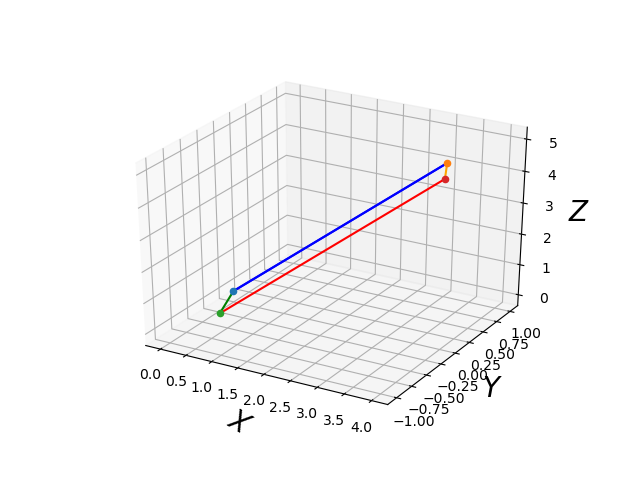
\includegraphics[width=\columnwidth]{./figs/parallelogram.png}
\caption{Parallelogram generated using python 3D-plot}
\label{fig:paral_sss_py}
\end{figure}

%
and the equivalent latex-tikz code generating Fig. \ref{fig:parallelogram1} is 
\begin{lstlisting}
figs/parallelo.tex
\end{lstlisting}
%
%The above latex code can be compiled as a standalone document as
%\begin{lstlisting}
%figs/triangle_fig.tex
%\end{lstlisting}

%

%

%
%

\end{enumerate}


